\documentclass{report}

\usepackage{tkz-orm}
\usepackage[utf8x]{inputenc}
\usepackage[frenchb]{babel}
\usepackage[T1]{fontenc}
\usepackage{lmodern}
\usepackage{fullpage}
\usepackage{graphicx}
\usepackage{epstopdf}
\usepackage{caption}
\usepackage{subcaption}
\usepackage{multirow}
\usepackage{framed}
\usepackage{eurosym}

\usepackage{multicol}

%Caractères spéciaux
\usepackage{pifont}
\usepackage[margin=2cm]{geometry}

% Affichage du graphique
\usepackage{tikz}
\usetikzlibrary{shapes, decorations.markings, shadows, arrows, positioning}
\usepackage{xcolor}

%inclure du code
\usepackage{listingsutf8}

% cfr http://en.wikibooks.org/wiki/LaTeX/Colors
\usepackage{color}
\usepackage{colortbl}
%\usepackage[usenames,dvipsnames,svgnames,table]{xcolor}
\definecolor{dkgreen}{rgb}{0.25,0.7,0.35}
\definecolor{dkred}{rgb}{0.7,0,0}

\usepackage{float}
\usepackage{pict2e}

\usepackage{listings}
\lstset{
  numbers=left,
  numberstyle=\tiny\color{gray},
  basicstyle=\rm\small\ttfamily,
  keywordstyle=\bfseries\color{dkred},
  frame=single,
  commentstyle=\color{gray}=small,
  stringstyle=\color{dkgreen},
  %backgroundcolor=\color{gray!10},
  %tabsize=2,
  rulecolor=\color{black!30},
  %title=\lstname,
  breaklines=true,
  framextopmargin=2pt,
  framexbottommargin=2pt,
  extendedchars=true,
  inputencoding=utf8x
}

\lstset{language={C}}


\newtheorem{theorem}{Theorem}[section]
\newtheorem{lemma}[theorem]{Lemma}
\newtheorem{proposition}[theorem]{Proposition}
\newtheorem{corollary}[theorem]{Corollary}

\newenvironment{proof}[1][Proof]{\begin{trivlist}
\item[\hskip \labelsep {\bfseries #1}]}{\end{trivlist}}
\newenvironment{definition}[1][Definition]{\begin{trivlist}
\item[\hskip \labelsep {\bfseries #1}]}{\end{trivlist}}
\newenvironment{example}[1][Example]{\begin{trivlist}
\item[\hskip \labelsep {\bfseries #1}]}{\end{trivlist}}
\newenvironment{remark}[1][Remark]{\begin{trivlist}
\item[\hskip \labelsep {\bfseries #1}]}{\end{trivlist}}

\newcommand{\qed}{\nobreak \ifvmode \relax \else
          \ifdim\lastskip<1.5em \hskip-\lastskip
                \hskip1.5em plus0em minus0.5em \fi \nobreak
                      \vrule height0.75em width0.5em depth0.25em\fi}


\colorlet{sblue}{blue!50}
\colorlet{sred}{red!50}
\colorlet{sgreen}{green!50}
\colorlet{syellow}{yellow!50}
\colorlet{spink}{dkgreen!50}

\usepackage{titlesec}
\titleformat{\chapter}
{\normalfont\LARGE\bfseries}{\thechapter}{1em}{}

\titlespacing*{\chapter}{0pt}{3.5ex plus 1ex minus .2ex}{2.3ex plus .2ex}
\setcounter{secnumdepth}{3} 
\begin{document}

\author{Houtain Nicolas}
\title{Synthese Network}

\maketitle
\tableofcontents

\chapter{Terminologie}

\begin{description}
    \item[DNS] : \textit{Domain Name System}. Service permettant de traduire un nom de domaine en informations de plusieurs types qui y sont associées, notamment une IP.
    \item[DIFS] : \textit{DCF Interframe Space}. Si une station détecte qu'il n'y a pas eu de transmission WiFi pendant DIFS microsecondes et que l'échange de la dernière trame a réussi, elle a le droit de transmettre. Cette valeur au sein de la gestion des collisions : DIFS = SIFS + (2 * Slot time)
    \item[EIFS] : \textit{Extended Interframe Space}. Similaire au DIFS mais activé uniquement si la dernière frame a échoué. EIFS = Temps de transmission d'un acquittement + SIFS + DIFS.
    \item[HTTP] : \textit{HyperText Transfer Protocol}
    \item[RIFS] : \textit{Reduced Interframe Space}. 
    \item[SDU] : \textit{Service Data Unit}
    \item[SIFS] : \textit{Short Inter Frame Spacing}. Temps pour une interface sans-fil entre la gestion d'une trame reçue et l'envoi de l'acquittement correspondant (temps pour passer de download à upload pour un routeur).  -> CSMA/CA
    \item[TLV] : \textit{Type Length Value} est un format d'encodage tel que le premier byte est le type, le second la taille totale et puis la valeur.
\end{description}


\chapter{Principles}

\section{Connecting two host}

By electrical cable, optical fiber, wireless.

\subsection{The physical layer}

\begin{description}
    \item[Bit rate] : Expressed in bits/sec
    \item[Bandwith] : Range of frequency usable 
\end{description}

He is not perfect (unreliable), and for us is like a black box with this characteristics :
\begin{itemize}
    \item may change a bit being transmitted
    \item may deliver more bits
    \item may deliver fewer bits
\end{itemize}

\subsubsection{Manchester encoding}
TODO page 8

\subsection{The datalink layer}

\begin{description}
    \item[Frame] : sequence of bit with a particular synthax or structure.
\end{description}

\subsubsection{Framing}

\begin{description}
    \item[Bit stuffing] : \textbf{01111110} is a frame boundary marker, so he can't
        be used when we transmitted frame. 
        \textit{Ajout un 0 pour assurer que ce marqueur n'est pas dans la frame}\\
        \begin{enumerate}
            \item Easy to implement in hardware.
            \item Increase number of bit transmited
        \end{enumerate}
\end{description}

\paragraph{Note} : Bit stuffing is implement in hardware and character stuffing is usually
implement in software.

\subsubsection{Reliable transfert}

On peut avoir plusieurs erreurs si on est trop lent à traiter les informations reçues
(\textbf{overflow} du buffer), si la frame est \textbf{perdue} ou à été \textbf{corrumpue}
par une erreur de transmission.

\paragraph{}
Two frames : \textbf{data frame} and \textbf{acknowledgment frame}.
Frame = Header (\textit{CRC or checksum} and \textit{frame number}) + Payload (\textit{data})

\paragraph{error detection}
 Hamming code \textit{is detection and correction error based on bit parity}, CRC 
 \textit{is powerfull to detect error}, checksum \textit{is really easy to use}.

\begin{multicols}{2} 
\subsection{Go-back-n}
\begin{itemize}
    \item N'accepte que les frames en séquence
    \item 0-$2^n -1$ numéro de séquences sont utilisé
    \item Ack contient la derniere frame reçue
\end{itemize}

\subsection{Selective-repeat}
\begin{itemize}
    \item N'accepte les frames hors-séquence
    \item 0-$2^{n-1}$ numéro de séquences sont utilisé
    \item Ack contient la derniere frame reçue (\textit{Utilisation du selective ack pour
            avoir des informations sur celle bien reçue hors-séquence})
\end{itemize}

\end{multicols}


\section{Building a network}
Host and router sending packet.

\subsection{The datagram organisation}

\subsubsection{Computing forwarding tables}
\begin{enumerate}
    \item Si on a un \textbf{tree-shapped network} il suffit d'inspecter les packets
        reçu pour créer sa table de forwarding sans risquer d'avoir de loop
    %TODO page 35
\end{enumerate}

\subsubsection{Flat or hierachical adresse}
Flat is like number telephone (small match to forwad packet) and hierachical is like a postal adress (smaller forwarding table, adress change when attached to other node\ldots question with mobile host).

\subsubsection{Dealing with heterogeneous datalink}
Page 39

\subsection{Vitual circuit organisation}

\subsection{The control plane}

\subsubsection{Distance vector routing}
%TODO

\subsubsection{Link state routing}
%TODO

\section{Application}
%Big-little indian


\section{The transport layer}

La couche de transport doit gérer les problèmes de la couche network :
\begin{itemize}
    \item corrupt data
    \item loose data
    \item not deliver data in-order
    \item upper bound on maximun length of the data
    \item duplicate data
\end{itemize}

\subsection{Connectionless}
On envoi les données et le service assure qu'elle arrive.
Utilisé pour le transport de petit SDU.

\begin{description}
    \item[Reliable] : Garantit l'arrivée à coup sur des données. (\textit{difficile à mettre en pratique})
    \item[Unreliable] : Imperfection :
        \begin{itemize}
            \item Garantit seulement une majorité qui arrive (\textit{Souvent ce qui est écarté est du à l'overflow du buffer})
            \item Peut duppliquer les packets sur le réseau
            \item Peut délivrer un SDU différrents
            \item A une taille limité des données
        \end{itemize}
\end{description}
% Characteristic page 56

\paragraph{Note:} Pour passer du network layer au transport layer, il faut ajouter la 
gestion des erreurs et une technique de multiplexing (\textit{via port}).


\subsection{Connection-oriented}
Ici il y a trois phases : établir la connection, transferer les SDUs (\textit{la connection est 
bidirectionnel}) et fermer la connection.

\begin{description}
    \item[Reliability] : Elle n'est garantie que lorsque la connection est terminé avec un
        ``gracefully``, sinon des pertes peuvent être observé
\end{description}

\subsubsection{Connection}

\paragraph{Refus:} Soit de la part du destinataire, soit du provider.

\paragraph{Three-way handshake} est utilisé contre l'approche naive de la connexion ``aller-retour''. Celle ci est définie par l'envoi d'un \textbf{CR}, répondu par \textbf{CA} qui répond \textbf{CA}.

Pour permettre le Three-way handshake, on utilise un transport clock.


\subsubsection{Data transfert}

\paragraph{Mode}
\textsc{message-mode} : On envoie et reçois les messages tels quels.\\
\textsc{stream-mode} : On envoit içi des flux de bytes, et on a besoin de spécifié un délimiter
spécifique pour déliumiter les SDU dans le bytestream.

$\rightarrow$  Le \textbf{Stream-mode}  est utilisé  pour les  reliable
transport portocols,  et le  numéro de séquence  placé dans  la frame
correspond à la position du premier byte du payload dans le bytestream.

\paragraph{Note} : Plusieurs différence par rapport au datalink layer pour assurer que les
données soient délivré. 

\begin{enumerate}  
    \item Dans  le datalink  layer quand  deux host  sont
connecté le délai de transmission est fixe. Ici le delai varie car les
paquets envoyés  ne prennent pas  forcément le  même path et  il peut
être mis en attente dans le buffer d'un router.
    \item Les paquets n'arrivent pas tjrs en séquence contrairement au datalink layer
    \item Le network peut duppliquer les paquets dans le transport layer
\end{enumerate}

\paragraph{Solution} :
\begin{enumerate}
    \item Pour détecter les erreurs de transmission, comme dans le datalink layer, on utilise un
    CRC ou checksum sur \textbf{chaque} segment.
    \item Pour rendre le protocole reliable, on utilise un numéro de séquence et des numéro
    d'ackowledgement. (32 ou 64bits nécessaire plutot que 8 dans les datalinks layer protocol)
\end{enumerate}

\paragraph{Go-back-n and selective repeat}
Dans le transport layer on va préférer le sélective repeat puisque cette couche 
ne garantit pas l'arrivée en séquence, contrairement au datalink layer.

De plus, dans le transport layer, plusieurs application concurrente peuvent communiquer
du coup l'espace mémoire offer à chaque application peut varier ce qui peut rendre la
taille du buffer variable.
Le sender à un swin (\textit{taille de son buffer}), et rwin (\textit{taille du buffer du receiver}). Il considère le minimun des deux comme la window size.


\textbf{Pour éviter un deadlock}, on utilise un persistent timer lorsque le sender reçoit une
window size du receiver égale à 0. Quand le timer expire on force le renvoi du dernier segment.

\subsubsection{Connection release}
Soit de manière \textbf{abrute}, soit de manière \textbf{gracefully} càd en fermant
les deux sens de la connections avec un DR suivit d'un ACK.


\subsection{Request-response service}

Page 61

\section{Naming and addressing}

\subsection{Benefit}

\section{Sharing ressources}

\textsc{bandwith} est la ressource la plus importante dans un réseau.\\
\textsc{buffer of network node} est une autre ressource importante.\\
\textsc{Processing capacity} to analyse packet and see on forwarding table.

\subsection{Organisation to sharing bandwith}

\paragraph{A full mesh}
Le plus efficace, mais nécessite $\frac{n \times (n-1)}{2}$ lien, et chaque 
host doit manager $n-1$ interface ce qui peut vite devenir impossible.

\paragraph{Bus organisation}
Le danger est que si le cable du bus est coupé en deux, le réseau est scindé
ce qui peut être dur à maintenir.

\paragraph{Star organisation}
Le noeud du centre de l'étoile est vital pour le réseau, mais il permet aussi
de centraliser le control en un seul point (\textit{C'est un excellent point de 
control et un bon point d'observation}).

Beaucoup plus facile à maintenir que le bus.


\paragraph{Ring organisation}
Un lien coupe l'entièrete du réseau, c'est pouquoi on utilise souvent un dual-ring.

\paragraph{Tree organisation}
Cela permet de connecté un large nombre de client avec un très petit coût.


\subsection{Sharing bandwith}

Le partage de bandwith dans les réseaux se veut être \textbf{max-min fairness}.

\paragraph{ }Plusieurs algorithme sont expliqué dans la section Medium Access Control.

\subsection{Network congestion}

Congestion lorsque $\sum demand > capacity$.

\paragraph{Congestion collapse}
Cela arrive lorsque le réseau est un peu congestionné, et donc la transmission est ralenti.
Si un protocole tel que \textsc{selective repeat} est utilisé, alors le sender peut
croire que le packet est perdu et donc renvoyé le packet ce qui ne fait qu'augmenter
la congestion! 


Pour régulere la congestion, une solution est de connaître la congestiona actuel afin que
les hosts ajuste leur bandwith disponible pour diminuer la congestion.

Tant que le buffer est peu ou pas du tout rempli, cela signifie que la demande est plus 
petite que la capacité et que le buffer sert juste à \textit{lisser} les demandes dans le temps.


\subsubsection{Discard mechanism}
On peut choisir d'écarter des paquets qd le buffer est full ou plutot quand il 
augmente dangereusement afin de prévenir une congestion!
Toutefois, discard a packet est la solution finale.

\begin{enumerate}
    \item Discard celui qui arrive. C'est le plus utilisé mais il tend à rester congestionner et
        les applications temps réelles en souffre bcp
    \item Discard le premier de la file est plus judicieux qu'il n'y parait puisque ce paquet
        y est depuis lgtps et on a surement déja détecté la perte (de part la congestion) avant!
    \item Random early discard permet de supprimer les paquets de différents flow en proportion
        à leur bandwith.
\end{enumerate}

Attention, supprimer un paquet est pas la meilleur solution puisqu'on supprime un paquet
qui a consommé des ressources alors qu'on manque justement de ressource!

\paragraph{Forward Explicit Congestion Notification}
Pour les réseaux datagramme, 
on utilise un bit pour marquer si le paquet est passé par un endroit congestionné,
et si c'est le cas le receiver envoi un paquet pour informer le sender du degré
de congestion (càd $\frac{nbr congestion}{nbr paquet}$)

\paragraph{Backward Explicit Congestion Notification}
Même technique pour les réseaux virtuels, sauf qu'on marque l'acknowledgement.

\paragraph{Control packet}
TODO

\subsubsection{Scheduler mechanism}
Permet d'attribuer une FIFO par flow et un round robin choisit le prochain paquet


\subsection{Distributing the load across the network}

\paragraph{Virtual network}
Ici lorsque un host veut envoyer une information, il spécifie la destination et parfois la
bandwith nécessaire. On lui répond si il peut ou non se connecter.. Cette technique
est utilisé notament par les téléphones.

\paragraph{Datagram network}
La technique du virtual ne peut être appliqué car dans le datagram un host n'a pas 
besoin d'autorisation pour envoyer des packets.

TODO page 82


\subsubsection{Shared popular file}

\paragraph{Save on multi server}

\paragraph{Using popular bittorent service}


\subsection{Medium Access Control Algorithms}

\textsc{Collisions} arrive quand deux host essaye d'envoyer simultanément une frame. 
C'est l'erreur principal sur les Local Area Network.

\paragraph{Deterministic or pessimist MAC} qui dit que les collisions sont la mort, et 
assure qu'il n'y en aura jamais.

\paragraph{Stochastic ou optimist MAC} qui est plus cool et minimise au maximun
les collisions.


\subsubsection{Static allocation methods}

\subsubsection{ALOHA}
Pour éviter d'avoir des collisions à la retransmission qd la transmission à échoué
par collision, chaque host attend un temps random avant de retransmettre par timeout.

De plus une excellente amélioration proposé ($perf \times 2$) est de ne pas permettre
que tout le monde retransmette quand il veut mais de donner à chaque host un timeslot
auquel il peut retransmettre.

\subsubsection{Carrier sense multiple access}
CSMA essaye d'améliorer ALOHA lorsque le résau est fortement utilisé.

Les host attendent que le channel soit libre avant d'envoyer une frame.

\paragraph{Persistent CSMA} L'attente que le channel soit libre constitue en soi
un point de synchronisation entre les hosts qui vont donc transmettre au même moment 
et provoquer des collisions. (Voir page 86)

\paragraph{Non-persistent CSMA} Propose lui d'écouter ponctuellement si il est libre
et le cas échéant d'attendre un temps random.

\subsubsection{Carrier sense multiple access with colision detection}


\subsubsection{Carrier sense multiple access with colision avoidance}
Utilisé pour le \textsc{wifi}, elle améliore le système de timeslot.

\textsc{sifs} est l'écart entre la reception et l'envoi de l'ack (\textit{du au switch upload/download du router})\\
\textsc{difs} 
\textsc{eifs}

TODO

\subsubsection{Deterministic medium access control algorithm}
TODO

\subsection{Congestion control}

Pour supprimer la \textbf{congestion collapse}, les hosts doivent réguler leur taux
de transmission. (\textit{Note qu'il y a d'autre méchanisme pour réguler tel que celui
basé sur les crédits})

Goals of congestion control for a set of i hosts :
\begin{itemize}
    \item Doit supprimer la congestion càd $\forall_t \sum r_i(t) \leq R$
    \item Efficace càd $\forall_t \sum r_i(t) \approx R$
    \item Juste pour tous (max-min fairness est l'utopie)
\end{itemize}

Le control de congestion est un algorithme qui adapte le taux de congestion :
\begin{enumerate}
    \item Multiplicative decreasing si il y congestion : $rate = rate*\beta, \beta <1$
    \item Additive increasing sinon :  $rate =  rate + \alpha, \alpha>0$
\end{enumerate}

\subsubsection{Congestion control in window-based transport protocol}
TODO

\section{The reference models}

\begin{description}
    \item[Application] : \textsc{SDU}
    \item[Transport] : connectionless/connection-oriented, \textbf{souvent unreliable}, \textsc{segment}
    \item[Network] : connect to network pas forcément directly, , \textsc{packet}
    \item[Datalink] : directly connect device, \textbf{reliable or unreliable}, \textsc{frame} with variable or fixed length
    \item[Physical] : directly connect device, \textbf{Unreliable}, \textsc{bit}
\end{description}


\chapter{Protocols}

\section{Application layer}
TODO

\section{DNS}
Structure DNS message page 113.

DNS permet d'obtenir l'adresse qui correpond à un certain nom, mais on peut 
faire un reverser DNS pour obtenir le nom d'une adresse.

\section{Electronic mail}

\subsection{Email message}
\textsc{Header:} (\textit{From, Date, To, Subject,  cc, bcc}) and \textsc{Body} 

Line to separate header and body is empty and contains only CR and LF.

\subsection{Header field to support Multipurpose Internet Mail Extension}
Header line :
\begin{itemize}
    \item MIME-version : version de MIME pour l'encodage du mail
    \item Content-type : Type de donnée du message
        \begin{enumerate}
            \item multipart/mixed : le fichier contietn des parties d'encodage
                indépendant (text, binaire séparé dans le body par une line vide)
            \item multipart/alternative : même message avec différentes représentation
        \end{enumerate}
    \item Content-transfert-encoding : Comment le message est encodé
\end{itemize}

\subsection{The Simple Mail Transfer Protocol}

\section{HTTP}
Utilise des liens hypertext pour lier un fichier à un autre.

\paragraph{Trois composant du world wide web}
\begin{enumerate}
    \item \textsc{uniform resource identifiers} : URI désigne une ressource sans aucune ambiguité 
sur le world wide web. (page 126)
    \item \textsc{html}
    \item Le protocol \textsc{http} composé de request (\textit{method, header, MIME document}) et response(\textit{status line, header, MIME document}).
\end{enumerate}

Page 129 pour les header fields.


Une requête \textsc{http} doit être \textbf{self-content}. Cependant, il est possible que
le serveur veulent personnaliser les réponses au préférence du client. Trois solution :
\begin{enumerate}
    \item En forçant le client à s'identifier (user/password is deprecated)
    \item TODO
    \item En utilisant des cookies
\end{enumerate}

\section{Remote Procedure call}
C'est comme appelé une procédure dans un code, sauf que l'on est pas sur
un host seul mais dans le réseau.

\paragraph{Encoding data}
\textsc{xdr} (\textit{plus efficace}), \textsc{json} (\textit{plus lisible}),\ldots

\paragraph{Reaching the calle}
Un mécanisme simple est \textsc{json-rpc} qui peut être utilisé en connectionless ou
connection-oriented, composé d'une requête et d'une réponse. (page 136)

\section{Internet transport protocols}
TODO page 137

\section{The User Datagram Protocol (UDP)}

C'est un unreliable connectionless transport service, au dessus d'une unreliable
connectionless network service, qui utilise les ports
pour permettre de communiquer avec plusieurs application et qui a comme
caractéristique :
\begin{itemize}
    \item SDUs doit être < 65467bytes
    \item Garantit pas que le SDU est délivré
    \item Ne peut pas délivré un SDU corrompu
\end{itemize}

\paragraph{Header} = Source port (16), dest port (16), length (16) et checksum (16)

\paragraph{Port} : 0 - 1023 (\textit{privileged}), 1024 - 49 151 (\textit{registered}),
49 152 - 65 535 (\textit{ephemere})

TODO paragraph page 139

\section{The transmission control protocol (TCP)}

Bi-directionnal bytestream d'une connection-oriented transport service, au dessus d'une unreliable connectionless network service.

(Window-based transport protocol using go-back-n)

\paragraph{Header} = Source port (16), dest port (16), sequence number (32), ack number (32), 
window size (16), checksum (16)

\subsection{TCP connection etablishment}
Three-way handshake utilisant sequence number, ack number et SYN flag.

\begin{figure}[h]
    \centering
    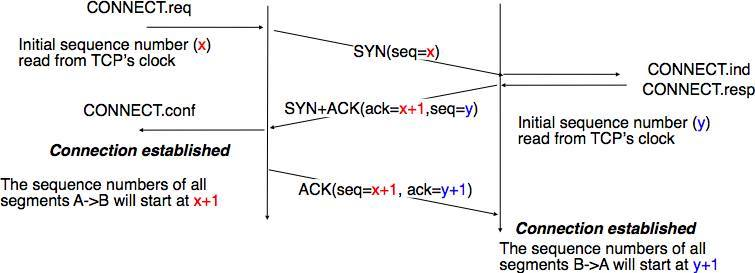
\includegraphics[width=10cm]{tcpconnect.jpg}
\caption{Connection TCP}
\end{figure}

Durant l'établissement de la connection, le client/serveur negocie plusieurs options :
\begin{enumerate}
    \item Le \textsc{mms} qui est la taille du plus grand payload acceptable (\textit{536 au minimun})
    \item La taille de la window
    \item L'utilisation de SACK
    \item Un ensemble d'option où client/server disent respectivemtn ce qu'il veut et ce 
        qu'il supporte
\end{enumerate}

\paragraph{Encodage des options} est fait en \textsc{TLV}.

\subsection{TCP reliable data transfert}

\subsubsection{Segment transmission strategie}

Deux solutions extrêmes :
\begin{enumerate}
    \item Première solution, envoyer quand on a besoin, mais cela peut impliquer d'envoyer
        un byte d'information avec 20 byte d'header\ldots pas très efficace
    \item L'autre extreme est d'envoyer qd on a rempli \textsc{mms} byte of data
\end{enumerate}

\paragraph{Nagle  algorithm}  :   on  envoi  le  paquet   si  il  rempli
un  \textsc{mms}  ou  si  l'on  vient  de  recevoir  un  acknwoledgement
(\textit{càd au moins à chaque round trip time}).

\subsection{TCP window}

La négociation du  window scaling factor ($0 \leq scaling  \leq 14$) se
fait  à la  connection, même  si certaines  implementations permettent
d'automatiquement ajuster la taille.

\subsection{TCP retransmission}
\textit{Go-back-n} a besoin d'un bon timer de retransmission (\textsc{rtt} est une
bonne estimation même si il change pdt la connection)

\textsc{rtt} = $\approx$ delai entre la transmission d'un segment et la reception de l'ack
\subsubsection{Measure RTT }
Le problème est que l'on ne sait pas de quel segment l'ack est la réponse (càd qu'il pourrait
y avoir plusieurs segment identique envoyé)

Pour cela on utilise le \textbf{timestamp option} :
\begin{itemize}
    \item \textsc{ts} : Par exemple valeur de la clock
    \item \textsc{ts} echo : Dernier \textsc{ts}val reçu\\
\end{itemize}


Comme y'a plus d'ambiguité, on peut mettre à jour la valeur du time (\textit{souvent à 3sec
de base}).

\begin{itemize}
    \item \textsc{srtt} (\textit{smoothed rtt mcomputed}) = $ (\alpha \times srtt) + (1-\alpha) \times rtt)$, $rtt$ est le \textsc{rtt} measured
    \item \textsc{rto} (\textit{retransmission timedout}) = $min(60, max(1, \beta \times srtt))$, 1 et 60 sont les bornes minimal/maximal
\end{itemize}

\paragraph{Jacobson's algorithm} : en pratique ça marche pas bien, donc jacobson a une
autre idée, il redéfini \textsc{rto} = $srtt + 4*rttvar$ avec \textsc{rttvar} = $(1-\beta) \times rttvar + \beta \times |srtt - rtt|$.

$\beta = \frac{1}{4}, \alpha = \frac{1}{8}$

\subsection{Advanced retranmission strategie}

\paragraph{}
\textsc{tcp} utilise de base \textbf{go-back-n}, et lorsque le même timer
expire on recommande de doubler le timer (appellé \textit{exponential backoff}) jusqu'à
ce qu'il ait atteint 60sec où le host est considée inateignable.

\paragraph{delayed acknowledgement strategy}
Par ailleurs, il est aussi possible de perdre bcp de performance en envoyant des
ack quand il n'ont pas bcp d'interet. Typiquement, il est possible d'implémenter
un \textbf{delayed acknowledgement strategy} qui assure d'envoyer un ack a chaque fin
de timer (\textit{delai cour}) ou si il reçoit un segment hors séquence puisque du coup
l'ack a énormément d'importance

\paragraph{Out-sequence}
Il est très facile pour le receiver d'ajouter un buffer pour récupérer les 
segments hors séquence sans avoir besoin d'en informer le sender.

\paragraph{Fast retransmit}
Actuellement, lorsqu'un segment est perdu il faut attendre que son timer expire
pour pouvoir le renvoyer. Une autre méthode consiste à détecter l'erreur lorsque
l'on reçoit 3 ack portant sur le même segment.

Il nécessite l'ajout d'une variable dubpacks dans le \textsc{tcb}.

\paragraph{Selective repeat}
Avec une option de TCP, on peut activer les \textbf{SACK} qui permettent d'indiquer 
les segments qui ont été reçu hors séquence. On utilise ici souvent Fast retransmit avec.

\subsection{TCP connection release}
Abrut (\textsc{rst}) ou gracefully.
TODO page 156

\section{The stream control transmission protocol (SCTP) }
Alternative au TCP qui offre :
\begin{enumerate}
    \item Supporte efficacement the \textit{multihomed host} càd avec plusieurs interface réseau. En TCP, une IP par interface et si tu te connecte en WIFI puis que ça
        crash la connection ne sait pas être reprise par la 3G.
    \item La possibilité de pouvoir envoyer des messages par bytestream
    \item Partially-reliable
    \item Une seule vrai connection avec des streams \textit{logique} pour éviter de manager
        plusieurs connection
\end{enumerate}

\subsection{Segment}
C'est un header suivit d'un ensemble de chunk.

\paragraph{Header} = Source port number (16), dest port number (16), verification tag (32) and checksum (32).

\paragraph{Chunk} = Type (8), flags (8), length (16) et value (32) pour permettre d'insérer facilement un ensemble d'option. STCP, contrairement à TCP, n'est pas limité sur le nombre d'option. C'est bon exemple de format de protocol facilement etendable.

\subsection{Connection etablishment}
C'est un four-way handshake (pour contrer l'attaque ``Denial attack'')

TODO image

\subsection{Reliable data transfert}

\paragraph{Data chunck}
Les données sont envoyé via des \textbf{data chunck} qui utilise un TNS comme 
numéro de séquence (augmenter de 1 a chaque data chunck). Lorsqu'un chunck est
scindé on utilise le bit \textsc{b} et \textsc{e} pour spécifier le premier et dernier
chunck.

\paragraph{Sack chunk}
Pour garantir l'arrivé, un TNS ack cumulatif est utilisé (Is on chunck level and not 
byte level). Il donne aussi des informations sur les chunck hors séquence.
Plusieurs autre différence :
\begin{enumerate}
    \item Il peut fournir de l'information sur différent ``trou'' dans le buffer de réception
    \item Il peut donner un feedback sur chunck dupplicate (Annonce une mauvaise heuristic du sender)
\end{enumerate}

\subsection{Connection release}
Applique un three-way handshake pour cloturer la connection.
TODO error

\section{Congestion control}
Le control est effectué dans la transport layer. 

\textsc{tcp} control la congestion en agissant sur la window size puisque une connection 
ne peut pas envoyer des données plus vite que $\frac{window}{rtt}$

\paragraph{Congestion window}
\textsc{cwnd} est stocké dans le \textsc{TCB} de chaque connection, et la taille de la window
est $min(cwnd, rwin, swin)$.  \textit{Additive increase} : Chaque \textsc{rount trip time}, on incremente \textsc{cwnd} de MSS byte. \textit{Multiplicative decrease} : Quand une congestion
est detecté on divise \textsc{cwnd}.

\paragraph{Initial value cwnd}
est de MSS bytes afin de ne pas congestionner le réseau au démarrage. 
(Cette valeur de départ à été augmenter à 15Kbyte)


Toutefois, cwnd va augmenter lentement avant d'arriver a une valeur qui utilise efficacement le
reseau. Pour éviter cela, on inclu un \textsc{slow-start algorithm} qui permet durant ce temps
de doubler \textsc{cwnd} chaque RTT.

\paragraph{Detect congestion} revient à detecter la perte de packet.
\begin{itemize}
    \item \textit{mild congestion} : Si on effecture un fast retransmit
    \item \textit{severe congestion} : Quand le timer de transmission expire
\end{itemize}

\begin{figure}
    %\includegraphics
    TODO image
   \caption{Congestion window with congestion}
\end{figure}

\subsection{Controlling congestion without losing data}
L'idée est de détecter avant la perte de paquet la futur congestion avec un 
\textbf{Explicit Congestion Notification}. (Quant un paquet passe par un router 
congestionné on met le bit à 1 et quand le receiver à cette information il la
transmet au sender pour adapter son débit)

\paragraph{}
\begin{enumerate}
    \item Pour déployer la solution, il faut un autre bit pour spécifier si le packet utilise
        ECN ou non. En effet, le cas échéant lorsque le router est congestionné ceux qui 
        n'implémente pas ECN sont avantagé
    \item Si le protocol est reliable ont peut informer le sender via l'ack. Soit via
        un flag dans le header soit via une option. TCP``choisi le flag, STCP l'option.
    \item Dernièrement, le sender/receiver savent si il utilise ECN via une TCP option
        durant le three-way handshake de connection
\end{enumerate}

Si le receiver detect une congestion, les prochain paquets envoyé auront cette information. 
(Pour éviter que l'information ne se perde si l'ack est perdu)

\subsubsection{Router algorithm}
Deux types de router, soit avec une FIFO soit un ensemble de FIFO et round robin scheduler.

Au lieu de prendre une mesure instantanée du remplissage du buffer, on prend une moyenne
du remplissage.
De plus, chaque paquet à une probabilité d'être marqué comme congestionné qui augmente
quand la moyenne augmente.

\paragraph{}
Quand il y a plusieurs queue ont fait cette probabilité de manière indépendante pour
garantir la justesse.

\subsection{Modeling TCP congestion control}
TODO

\section{Network layer}
Trois type de datalink layer :
\begin{enumerate}
    \item Utilise directement le lien physique du physical layer
    \item Utilise un Local Area Network
    \item Utilise un Non-Broadcast Multi-Access (utilisé pour simuler une LAN supportant
        juste l'unicast)
\end{enumerate}

\paragraph{LAN} Dans une LAN Chaque host est identifié par un datalink layer adresse
(\textbf{MAC adresse}). 
LAN supporte broadcast and multicast datalink layer adresses. Une frame envoyé a l'adresse
broadcast/multicast de la LAN est envoyé à tout les participants/participants correspondant
au groupe.

\subsection{IP version 6}
IPv4 ne pourra bientot plus supporter toute les adresses, d'ou le besoin
de passer à une autre solution.

\subsubsection{IPv6 adressing architecture}
Support unicast, multicast and anycast.

\subsubsection{Unicast}
TODO image 171

Une allocation hierarchique des allocations d'adresse permet de minimiser
le nombre de route connu par les router. Celui ci connait donc pour
certains block d'adresse!

$2^{128}$ groupé dans $2^{64}$ subnet!


Deux type d'allocation d'adresse :
\begin{enumerate}
    \item \textit{provider independent} (PI) 
    \item \textit{provider aggregatable} (PA) 
\end{enumerate}
TODO understand

\paragraph{Size IPv6 adress}
/32 = Internet Service Provider, /48 = single compagny, /56 = small user site,
/64 = single user, /128 = rare (Pas plus d'un host attaché au prefix)

\paragraph{Utilisation IPv6 prefix}
\textit{Longest prefix match} assure que la route qui match le plus avec
l'adresse est celle employé. 

Note : ::/0 match avec tout le monde et est donc la \textit{default route}.

\paragraph{Link local unicast}
L'addresse commence par fe80::/64 et est suivi des 64 bits d'interfaces.
Utilisé quand deux host sur le même lien (or LAN) veulent échanger des
packet.. Note que le router ne peut pas forwarder un packet avec un
link local unicast.
(Utilisé qd on ne peut pas avoir une IPv6 régulière, càd en LAN isolé)


\subsubsection{Multicast}
Envoyé efficacement un packet à toute les personnes d'une même groupe, dans une LAN.
TODO

\subsubsection{IPv6 packet format}

\paragraph{No checksum}
Il n'y a pas de checksum dans le header de packet IPv6 car il y a déja le checksum
sur les frame au niveau datalink layer! En pratique, l'ajout d'un tel checksum prévient
les erreur de corruption de mémoire au sein d'un routeur (\textit{ridicule}) pour un coùt de
calcule élevé.

\paragraph{Next header}
Indique le prochain header, tel que un transport layer header (UDP, TCP, SCTP) ou une
IPv6 option (page 177). Note qu'une option a aussi le champ \textit{next header}.

\paragraph{Fragment option}
En IPv6 la fragmentation est fait par le sender et non par le router. (Celui-ci discard
le paquet et envoi un message d'erreur au sender si le packet est trop grand).

Un paquet fragmenté contient un numéro d'offset de la fragmentation, le next header (car une option), un champ réservé mis à 0, un flag pour dire si c'est le dernier fragment et un
champ pour \textit{identifier} le packet original.

\subparagraph{Note:} On peut envoyer les packets du premier au dernier ou dans l'ordre inverse.
La deuxieme solution permet au receiver de connaître la taille du paquet (et donc du buffer
nécessaire).

\subsection{ICMP version 6}
\textit{Internet Control Message Protocol} version 6 est utilisé dans un paquet IPv6 
(next header = 58). Deux type de messages :

\begin{itemize}
    \item Messages d'erreurs 
        \begin{enumerate}
            \item Destination unreachable (0: no route, 1: firewall refuse, 2: sender use link-local adresse to reach global unicast adresss, 3: adress unreachable, 4: port unreachable)
            \item Packet too big
            \item Time exceeded
            \item Parameter problem
        \end{enumerate}
    \item Messages d'information
\end{itemize}
TODO page 184

\section{The IPv6 subnet}
TODO

\subsection{Interactions between IPv6 and datalink layer}

Dans une LAN sans internet, les hosts prennent une adresse IP grace au link-local adresse.
Si la LAN est connecté à internet, on utilise \textit{Neighbor Discovery Protocol} (partie de ICMPv6) pour connaître l'adresse des autres

\subsubsection{Neighbor Discovery Protocol}

\begin{enumerate}
    \item Envoi un multicast ICMPv6 Neighbor Solicitation avec son adresse IPv6
    \item Le receiver répond avec un ICMPv6 Neighbor Advertisement avec son adresse IPv6 et MAC
    \item En recevant le ICMPv6 NA, il stock le lien IPv6-MAC dans sa NDP table
\end{enumerate}
ICMPv6 NS peut aussi être utilisé pour voir si un host est atteignable. De plus, le ICMPv6 NA est
stocké temporairement dans la cache et quand il expire il faut revalider l'adresse.

\subparagraph{ }
\textit{Duplicate Address Detection algorithm} permet de ne pas avoir deux adresses identiques.
Pour cela il envoit un ICMPv7 NS à sonn adresse, et si il ne reçoit pas de réponse elle est
donc unique.

\subsubsection{Automatically configure IPv6 adress}
\paragraph{Stateless Address Autoconfiguration} mechanism obtient sa link-local adresse
en prenant 64 bits concaténé avec fe80::/64 et en verifiant avec un NS son unicité.

\paragraph{ }
Obtenir  une   vrai  adresse  est   effectué  en  envoyant   un  Router
Advertissement  message  à  ff02::1  qui est  accessible  à  tout  les
local-link adresse.

\subparagraph{Option}
TODO page 189

\paragraph{Dynamic Host Configuration Protocol} (DHCP)
TODO

\subsubsection{Multi router on subnet}
TODO



TODO image 189

\section{Routing in IP networks}
Deux classe de protocol entre les différents domaines pour echanger
efficacement de l'information.

Une grande différence entre intra et inter domaine est la \textit{routing policies}
utilisé par chaque domaine.

Dans un domaine toute les routers sont égaux et la meilleur route est choisi sur
différents critére : temps, nombre d'intermédiare et taille de bandwith.

\paragraph{Routing  policies}  =  import filter  (spécifie  les  routes
acceptables), export  filter (spécifies  les routes dangereuses)  et un
algorithme qui choisi.


\section{Intradomain routing}
Echange des informations sur les destinations atteignables \textbf{dans} le domain.
\textit{RIP} est protocol de distance vector et \textit{OSPF} utilise link-state routing.

\subsection{RIP}
Les routers echanges periodiquement des RIP messages (inside UDP segment).
Pour accélerer le processus (qd un router boot), il peut envoyer une RIP request à ff02::9 
pour demander tout de suite les tables de routings (reçu via un RIP response).

\paragraph{RIP response} contiennent les distance vectors des tabels de routing.

\subsection{OSPF}

\subsubsection{Area}
Avec le link-state routing, pour des grands réseaux c'est très couteux de stocker
l'ensemble du réseau en mémoire. C'est pourquoi on décompose le réseau en un 
ensemble d'\textsc{area} où les routers connaissent la topologie de sa propre
région et comment rejoindre la \textit{backbone area}

\paragraph{Backbone area}
C'est l'area qui regroupe tout les \textit{border router} et ceux qui sont relié
à ces routers sans être dans une area.

L'inter-area routing est fait via un distance vector protocol.

TODO image page 195

\subsubsection{LAN}
TODO point to point (R8-RC ? )

\subsubsection{Shortest path}
TODO page 196

\section{Interdomain routing}
Echange de l'informations entre les domaines. Cette information est une information
agrégé des routers et on considère ici les domaines comme des boîtes noires.

\subsection{Connection}

\paragraph{Private peering link} permet de lier deux domaines. Pour des questions
de performances plusieurs lien physique sont établi entre les domaines.

\paragraph{Internet eXchange Point} Une solution moins couteuse est de les connecter
via un IXP. TODO page 198

\subsection{Connection cost} Le coût d'une route est très importante en interdomain
alors qu'en intra on préfére la performance.

Il existe deux types de relation entre domaine \textit{customer->provider} et \textit{
shared cost}.
TODO image page 198

\paragraph{customer->provider}
Le customer paye pour que son domaine soit distribué dans Internet

\paragraph{Shared cost}
Cela arrive quand on a des domaines de taille similaire 

\paragraph{Sibling}
Ils échangenet les routes dans les deux directions (souvent c'est des routers
de la même compagnie).

\subsection{Interdomain routing policie}
TODO

\subsection{The Border Gateway Protocol (BGP)}
Dans BGP chaque domain est identifié par un unique \textit{Autonomous System} number (AS).

BGP n'envois pas sa routing table entière mais le fait de manière incrémentale, càd en
envoyant uniquement les routes qui ont changé.

De plus BGP utilise TCP pour garantir le bon délivrement des BGP messages.

\subsubsection{BGP session}

\paragraph{Etablisment} doit être fait manuellement pour des raisons de sécurité.

\paragraph{Messages}

\begin{enumerate}
    \item \textit{OPEN} : Quand la connection est établie, ça initialise la session et
        négocie d'option
    \item \textit{NOTIFICATION} : Pour cloturer la session
    \item \textit{UPDATE} : Averti du changement d'une route. C'est le message le plus important et pour que le protocol soit efficace, le message doit minimiser le nombre de bit envoyé.
    \item \textit{KEEP ALIVE} : Averti que rien n'a changé (pour être sur que le router
        est toujours en vie)
\end{enumerate}

\paragraph{BGP update} = \{IP prefixe retié\}, \{IP préfixe ajouté\}, \{AS-Path\}

\subparagraph{ } Une route qui est envoyé doit d'abord passer l'\textit{export filter},
de même qu'une route reçue doit passer l'\textit{import filter}.
TODO

\subsubsection{The BGP decision process}
En plus des import/export filter, il y a un algorithme qui choisit la meilleur route.
Ce choix est fait sur base des BGP attribut attaché à chaque route.

\paragraph{Local-pref} 
Le premier attribut de cet algorithme est la local-preference, celui ci est attribué
selon l'import filter. (Highest value est préféré)

\subparagraph{Cheap link} On peut implémenté la préférence d'un lien peut couteux
plutôt qu'un autre via le local-pref en définissant les valeurs dans l'import filter.


\paragraph{Local-pref with customer->provider and shared cost}
\begin{enumerate}
    \item High local-pref pour les routes apprisent par le customer (\textit{provider->customer})
    \item Medium local-pref pour les shared-cose
    \item Low local-pref pour les routes apprisent par le provider (\textit{customer->provider})
\end{enumerate}


\subsubsection{BGP convergence}
Certaines routing policies peuvent interférer entre elles et aboutir (en théorie), 
à des ping-pong infini.

\paragraph{ } La convergence des BGP n'esy pas toujours garanti et verifier la 
convergence global est un problème NP-complet.

\paragraph{Guideline to guarantee BGP convergence}
\begin{enumerate}
    \item Le graph est \textit{customer->provider} est acyclique
    \item AS préfére une route reçue d'un customer plutôt qu'une shared-cost
\end{enumerate}

\subsection{Structure global internet}
TODO page 209

\section{Datalink layer technologie}

\subsection{The point to point protocol}
Protocol dévellopé après me \textit{Serial Line IP} (SLIP) qui a beaucoup de limitation.

PPP est enfaite en famille de trois protocol :
\begin{enumerate}
    \item The PPP define framing technique to transport network layer packet
    \item The \textit{Link Control Protocol} est utilisé pour negociate option and authentification by username/password
    \item The \textit{Network Control Protocol} est spécifique à chaque network layer protocol
\end{enumerate}

PPP frame utilise le bit/caractère stuffing, supporte variable length (même si LCP négocie la MAX size).

\subsection{Ethernet}
TODO changement + slot time

\paragraph{Hubs}
Les hosts peuvent être directement relié à un Ethernet hubs. 
\subparagraph{Complexe network hub} La topologie doit être un tree et le délai entre
deux host ne peut pas être plus long que 51.2ms (slot time).

\subsubsection{Frame format}
TODO image page 213

\subsubsection{Ethernet service}
Ethernet network offre un unreliable connectionless service qui supporte unicast, multicast et
broadcast.

En pratique il délivre les frames au destinataire avec une \textbf{TRES} grande probabilité,
et les frames arrivent en séquence.

\subsubsection{Fast ethernet}
TODO page 215

\subsubsection{Ethernet switches}
Augmenter la bande passante comme \textit{fast ethernet} n'est pas la seule 
manière d'améliorer les performances d'ethernet LAN, on peut aussi rendre
les hubs intelligents en devenant des switchs.

Ceux-ci maintiennent une table de forwading pour les MAC adresses.

TODO image page 217


\paragraph{MAc adress}
Quand deux host sont sur le même hub/segment ethernet, ils peuvent échanger de 
l'information sans configuration ce qui implique que un switche doit pouvoir 
construire sa table de MAC adresse \textit{automatiquement}.

$\rightarrow$ Pour chaque frame reçue, la MAC adress est extraite de la frame et mise dans la table.

\paragraph{ }
The \textit{MAC adress learning} algorithm fonctionne bien sur un tree-shaped network,
sauf que cette topologie est dangereuse si l'un des switchs tombent en panne\ldots

Toutefois, si ce n'est pas un arbre ont peu rapidement tomber dans une boucle infinie
(si il n'y a pas de RTT ou Hop limit)!

\subsubsection{Spanning tree protocol}
Désactive automatiquement des ports pour rester dans une tree-shaped, mais si l'un
des switchs crash, il y a un autre qui peut prendre le relais.

Le switch root est celui avec la plus petite MAC adress, ensuite le spanning tree est construit
pour que chaque switch ait le plus path vers le root.

Ils utilisent des BPDUs qui contiennent :
\begin{itemize}
    \item L'identifiant du root
    \item Le coût du path entre le root et celui qui envoit le BPDU
    \item L'identifiant de celui qui envoit le BPDU
    \item Le nombre de switch port par lequel il est passé
\end{itemize}


Durant la création du spanning tree toutes les data frames sont écarté 
car on ne peut pas garantir l'absence de loop.


\subsubsection{Virtual LAN}

TODO page 222

\subsection{802.11 Wireless networks}

TODO page 223



\end{document}
